% !TeX spellcheck = da_DK
\subsection{Forstærker i opsamlingsblok}\label{Subsec:Forstaerker}
\subsubsection{Teori og design}
Til forstærkningen i opsamlingsblokken på \figref{kravblok} skal der benyttes en ikke-inverterende forstærker, da der ønskes, at inputtet og outputtet har samme polaritet. Ved en ikke-inverterende forstærker bliver inputtet tilkoblet direkte til den ikke-inverterende inputterminal, hvilket vil give en høj inputimpedansen, da der kigges direkte ind i operationsforstærkeren. Kredsløbet består af en operationsforstærker kaldet LT1028A, som ligner den operationsforstærker, der er tiltænkt at benytte i implementeringsdelen. Denne sidder i et closed-loop med modstandene R$1$ og R$2$, som udgør en spændingsdeler. Dette ses på \figref{fig:Forstaerker}.
\begin{figure}[H]
\centering
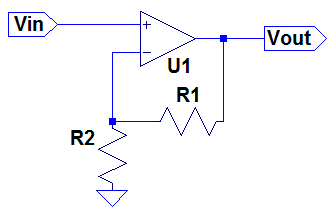
\includegraphics[scale=0.85]{figures/cProblemloesning/Forstaerker.PNG}
\caption{Kredsløbet for en ikke-inverterende forstærker i en closed-loop konfiguration.}
\label{fig:Forstaerker}
\end{figure} 

\noindent Der er jævnført i afsnit \ref{OpsamlingsAfs} på side \pageref{OpsamlingsAfs} bestemt, at forstærkningen skal være en faktor $18$, hvilket svarer til $25.1055$dB. For at udregne modstandene er R$2$ blevet valgt til $10$K$\Omega$. Ud fra dette er R$1$ blevet bestemt ved følgende udregning:
\begin{align}
18 = 1 + (\frac{R1}{10\text{K}\Omega})\\
R1 = 170\text{K}\Omega
\end{align}

\noindent R$1$ og R$2$ bliver brugt til at designe kredsløbet for en ikke-inverterende operations forstærker. Dette kredsløb designes i LT-spice, som ses på \figref{fig:Forstaerker_faktor18}. 
\begin{figure}[H]
\centering
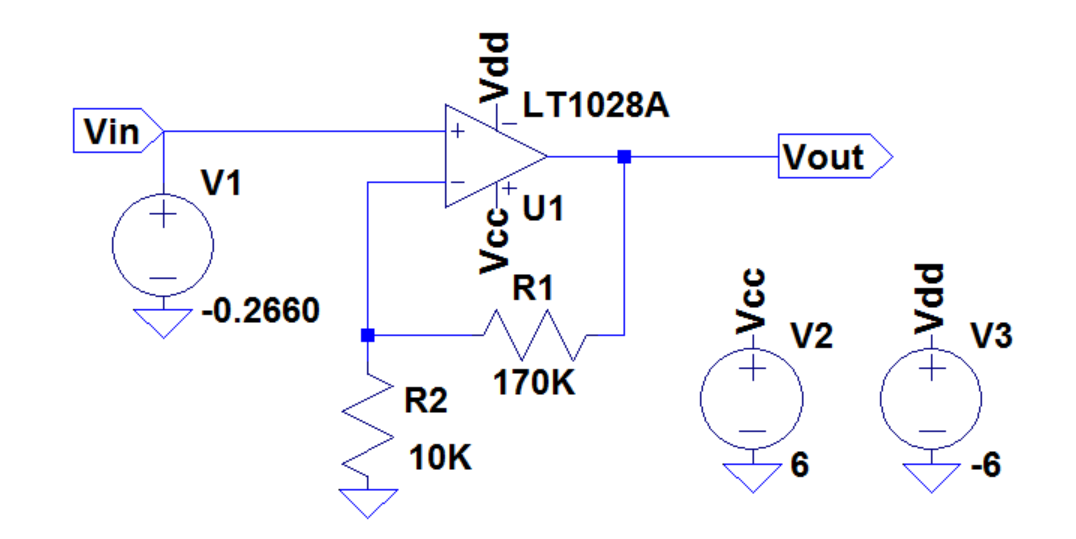
\includegraphics[scale=0.5]{figures/cProblemloesning/Forstaerker_faktor18.PNG}
\caption{Kredsløbet for en ikke-inverterende forstærker med to modstande, R$1$ og R$2$, som med værdierne $10$K$\Omega$ og $170$K$\Omega$ giver en forstærkning med en faktor $18$.}
\label{fig:Forstaerker_faktor18}
\end{figure} 

\subsubsection{Simulering}\label{Subsec:Forstaerker_simu}
Der undersøges i tre simuleringer, om forstærkeren virker ved det laveste input på -$0.2660$V, uden påvirkning ved $0$V samt højeste input på $0.2712$V. Det kan ses på \figref{fig:Forstaerker_faktor18_simulering}, at det forstærkede signal, kaldet $V_{out}$, er ca. $0.2712$V, hvilket er $18$ gange større end $V_{in}$, som i simuleringen er sat til $0.2712$V. Derved er der sket den ønskede forstærkning, hvilket var forventet, da simuleringen er med ideelle komponenter. Derfor har de enkelte komponenter ingen tolerance, som der vil være ved reelle komponenter i et reelt kredsløb. \\. 

\begin{figure}[H]
\centering
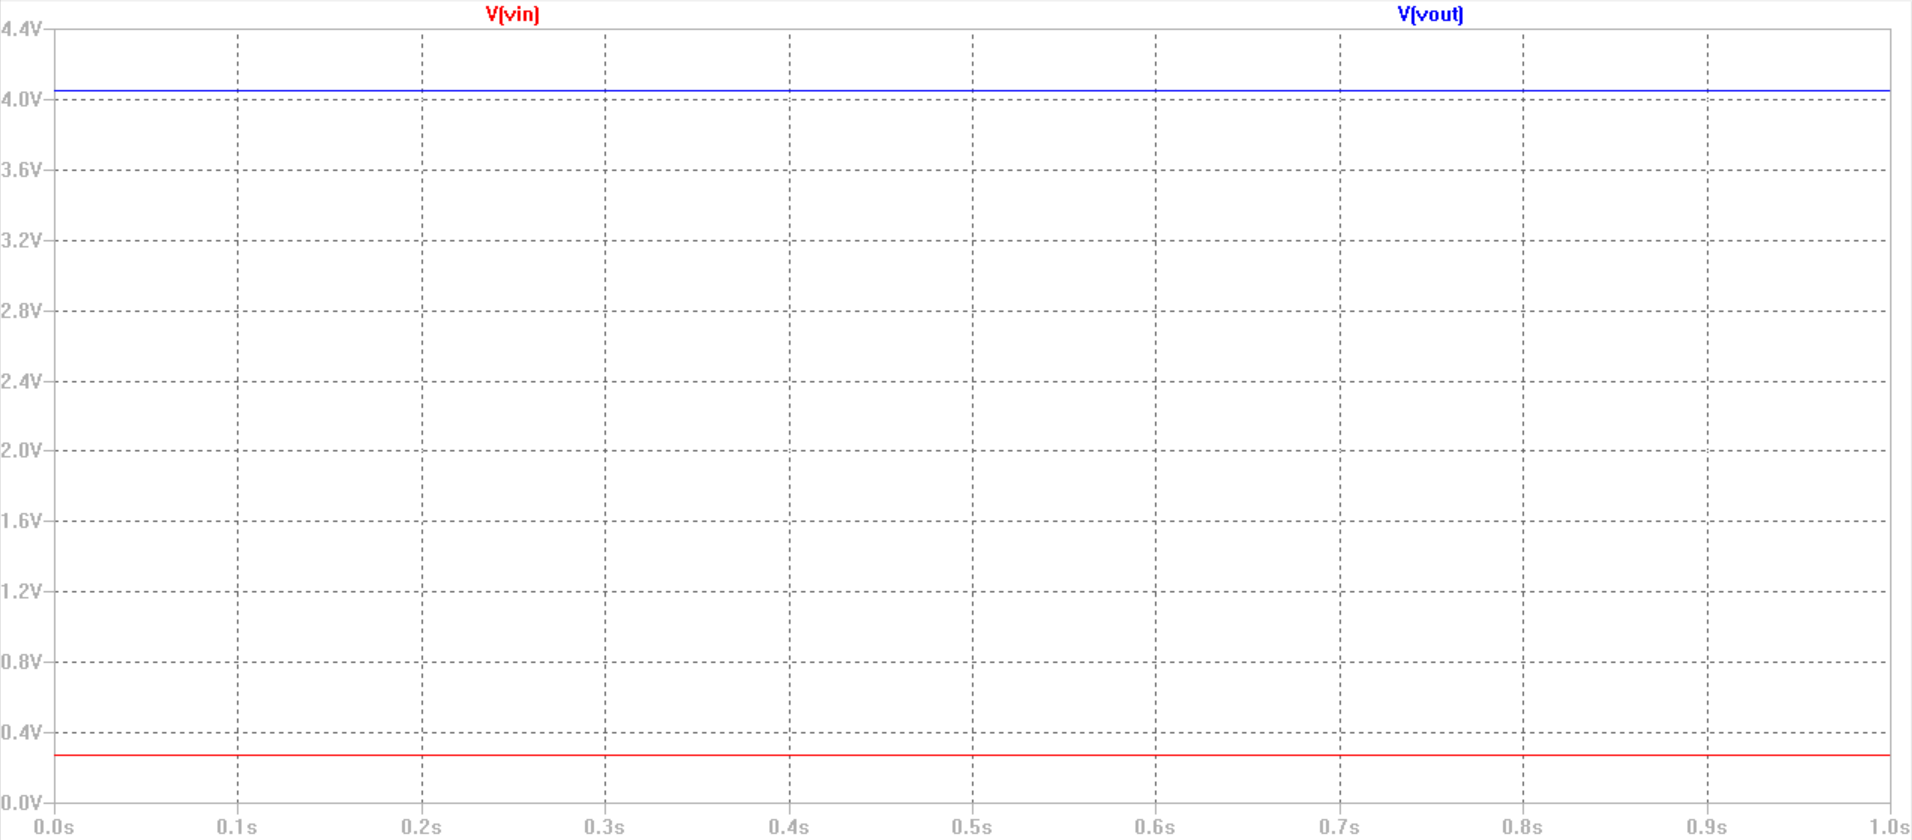
\includegraphics[scale=0.4]{figures/cProblemloesning/Forstaerker_faktor18_simulering.PNG}
\caption{En simuleringen af en ikke-inverterende forstærker, som ses på \figref{fig:Forstaerker_faktor18}, hvor der er en forstærkning med en faktor $18$. Dette kan på figuren ses at inputtet, $V_{in}$, er $0.2712$V, som bliver forstærket $18$ gange}
\label{fig:Forstaerker_faktor18_simulering}
\end{figure}

Resultaterne af de tre simuleringer ses i \tableref{tab:forstarker18_sim}
\begin{table}[H]
	\centering
	\begin{tabular}{|l|l|l|l|l|}
		\hline
		\multicolumn{1}{|c|}{\textit{Inputsignalet}} & \multicolumn{1}{c|}{\textit{Forstærkning}} & \multicolumn{1}{c|}{\textit{Forventet outputsignal}} & \multicolumn{1}{c|}{Outputsignalet} & \multicolumn{1}{c|}{\textit{Afvigelse}} \\ \hline
		$0.2712$V      & 18       & $4.8816$V     & $4.8817$V    & $0.0020\%$  \\ \hline
		$0$V           & 18       & $0$V          & $0$V         & $0$\%       \\ \hline
		-$0.2660$V     & 18       & -$4.7880$V    & -$4.7881$V   & $0.0020\%$  \\ \hline
	\end{tabular}
	\caption{Her ses resultaterne for simuleringerne med det laveste input, uden påvirkning samt højeste input.}
	\label{tab:forstarker18_sim}
\end{table}
Der ses på afvigelserne, at der arbejdes med ideelle komponenter, da der er en meget lav afvigelse i outputtet ift. det forventede output. Den procent mæssige afvigelse holder sig derved inden for tolerancekravene beskrevet i afsnit \ref{OpsamlingsAfs} på side \pageref{OpsamlingsAfs}.

\subsubsection{Implementering og test}